% !TeX spellcheck = pt_PT
%
% Classe do documento e parâmetros gerais.
\documentclass[a4paper,openright,twoside,11pt]{report}

% Packages utilizadas e respetivos parâmetros.
\usepackage[utf8]{inputenc}
\usepackage[portuguese]{babel}
\addto{\captionsportuguese}{\renewcommand{\bibname}{Refer\^{e}ncias}}
\addto{\captionsportuguese}{\renewcommand{\contentsname}{\'{I}ndice}}
\addto{\captionsportuguese}{\renewcommand{\appendixname}{Ap\^{e}ndice}}

\usepackage{lipsum} % gerador de texto
\usepackage{graphicx}
\usepackage{url}
\usepackage[Algoritmo]{algorithm}
\usepackage{algorithmicx}
\usepackage{algpseudocode}
\renewcommand{\algorithmicrequire}{\textbf{Dados: }}
\renewcommand{\algorithmicensure}{\textbf{Resultado: }}

% Definições das dimensões das páginas
\setlength{\textheight}{24.00cm}
\setlength{\textwidth}{15.50cm}
\setlength{\topmargin}{0.35cm}
\setlength{\headheight}{0cm}
\setlength{\headsep}{0cm}
\setlength{\oddsidemargin}{0.25cm}
\setlength{\evensidemargin}{0.25cm}

%\renewcommand{\baselinestretch}{1}

% Página inicial (capa)
\title{
   \vspace{-50mm}
   \begin{minipage}[l]{\textwidth}
      \hspace{-20mm}\resizebox{75mm}{!}{
\includegraphics{./figures/logoISEL.png}}\\
   \end{minipage}\\[20mm]
   {\bf RugbyApp}
}

% Nome dos autores (um por linha)
\author{
\begin{tabular}{ll}
             & Rui Garcia  \\
             & João Ferreira \\[50mm]
\end{tabular}}

\date{
\begin{tabular}{ll}
  	{Orientador:} & Jorge Martins \\
\end{tabular}\\[10mm]
% Deixar o indicador respetivo em função da versão do relatório.
Relatório de progresso realizado no âmbito de Projeto e Seminário\\
Licenciatura em Engenharia Informática e de Computadores\\[20mm]
Maio de 2020}


\begin{document}
\pagenumbering{roman}
\thispagestyle{empty}
\maketitle

\baselineskip 18pt 

\newpage
\thispagestyle{empty}
\cleardoublepage
\setcounter{page}{1}
\begin{center}
\textsc{\LARGE Instituto Superior de Engenharia de Lisboa}\\[50mm]

{\large \bf  RugbyApp}\\[20mm]

\begin{tabular}{rl}
  40539  & Rui Miguel Marques Garcia\\[10mm]
           & \rule{75mm}{0.5pt}\\[5mm]
  40913  & João Carlos Máximo Ferreira\\[10mm]
           & \rule{75mm}{0.5pt}\\
\end{tabular}\\[10mm]

\begin{tabular}{rl}
  Orientador & Jorge Manuel Rodrigues Martins Pião\\[10mm]
              & \rule{75mm}{0.5pt}\\[5mm]
\end{tabular}\\[10mm]

Relatório de progresso realizado no âmbito de Projeto e Seminário\\
Licenciatura em Engenharia Informática e de Computadores\\[20mm]
Maio de 2020\\
\end{center}

\cleardoublepage
\chapter*{Resumo}
O Rugby é um desporto que representa uma grande presença no quotidiano dos membros do nosso grupo, por sermos ou conhecermos praticantes ativos, e experienciamos a maioria das vertentes deste desporto há um longo período de tempo. A falta de presença deste desporto no conceito geral da nossa cultura não o expõe a tanto apoio e auxílio como noutros desportos de grande renome, o que se constata de forma clara, sem a necessidade de uma busca intensiva. 

A ideia deste projeto nasceu da nossa própria necessidade de criar uma aplicação que preencha essa lacuna. Com o foco primário em trazer às equipas deste desporto uma aplicação virada para a organização e gestão de informação dentro duma equipa, esperamos no fim apresentar uma ferramenta que consiga aglomerar os aspectos principais de uma equipa num único sitio, e que proporcione um apoio extra à maioria das suas necessidades funcionais.

%{\bf Palavras-chave:} lista de palavras-chave separadas por ;.

%% Página de agradecimentos
\cleardoublepage
\chapter*{Agradecimentos}
Agradecemos às equipas técnicas do Belas Rugby Clube e do Sporting Clube de Portugal pela disposição e partilha de ideias e comentários, afim de atenuar a ideia principal em que se baseia este projeto. Agradecemos também ao engenheiro Jorge Martins por se disponibilizar para ser o nosso orientador do projeto.
%Texto dos agradecimentos. É opcional.\\

% Geração do índice de conteúdos
\cleardoublepage
\tableofcontents \cleardoublepage

% Geração do índice de figuras e de tabelas
%\listoffigures \cleardoublepage
%\listoftables \cleardoublepage

% Reiniciar a numeração de páginas
\setcounter{page}{1}
\pagenumbering{arabic}

% Capitulo 1
% !TeX spellcheck = pt_PT
%
%
% Capítulo 5
%
\chapter{Introdução} \label{cap:intro}

Este projeto foi desenvolvido no âmbito de Projeto e Seminário, no semestre de Verão de 2020 da Licenciatura em Engenharia Informática e de Computadores. 
Este capítulo está organizado em três secções que descrevem o enquadramento e objectivo do projeto, assim como a organização do documento.


%
% Secção 1.1
%
\section{Enquadramento\label{key}} \label{sec11}

%
%Texto da secção. Na figura~\ref{fig:logotipo} mostra-se o logótipo do ISEL. Em \cite{wiki:bigdata2019} encontra várias referências para o assunto. O artigo \cite{6547630} é o mais popular conforme indicação do IEEE. Logo a seguir aparece \cite{6824752}. A identificação das referências deve ser melhorada.
Este projeto tem como temática principal o desporto Rugby. Sendo uma atividade desportiva pouco reconhecida ou relevante no contexto da nossa cultura, é notória a falta de ferramentas que proporcionem suporte à pratica desta atividade. Este problema foi apresentado aos diversos elementos do grupo devido a ligações interpessoais entre estes e o desporto, experienciando ativamente e lidando com este problema no próprio quotidiano.

Apesar de existir um grupo de ferramentas que proporcionem uma melhor qualidade na organização e prática desta modalidade, este foi considerado pelos estudantes como um grupo escasso e dispendioso, pelo que foi optado como objectivo deste projeto criar uma aplicação que assente na ideia de ajudar ativamente equipas técnicas desta modalidade desportiva em vários temas relevantes à otimização e melhoria do desempenho da equipa ao longo da época desportiva.

% Colocar uma figura
%\begin{figure}[h]
%\begin{center}
%\resizebox{100mm}{!}{
\includegraphics{./figures/logoISEL.png}}
%\end{center}
%\caption{Legenda da figura com o logótipo do ISEL.}\label{fig:logotipo}
%\end{figure}

%Continuação do texto depois do parágrafo que refere a figura.

%
% Secção 1.2
%
\section{Objetivos e Funcionalidades}\label{sec12} 

Esta secção aborda os objetivos e funcionalidades principais e secundários. É de notar que entre a proposta de projeto inicial e o corrente relatório ocorreram diversas reuniões com as equipas técnicas do Belas Rugby Clube e Sporting Clube de Portugal, pelo que é notável alguma diversidade de objetivos entre ambos os documentos.

A ideia chave deste projeto é criar uma aplicação que seja capaz de recolher e analisar estatisticamente dados sobre o desempenho dos jogadores de uma equipa de Rugby, afim de monitorizar aspetos críticos que avaliem não só o estado individual de cada jogador, como o estado atual de toda a equipa. Pressupõe-se que toda a informação recolhida consiga facilitar aspetos chaves do funcionamento de uma equipa desportiva, auxiliando desde a face tática do desporto (aspetos como a constituição da equipa, o plano tático, a otimização de temáticas de treino), assim como a face menos técnica de uma equipa (aspetos como a organização de treinos e jogos, a facilidade de acesso a informação pertinente, entre outros).

Pretende-se aglomerar todos estes aspetos numa única aplicação, que ofereça aos utilizadores, sendo eles atletas ou equipa técnica, uma plataforma onde possam observar os dados aglomerados referentes a cada jogador em particular, os dados referentes a jogos concretos ao longo da época, aceder a planos de treinos físicos propostos pela equipa técnica, e observar uma linha temporal sobre todos os eventos futuros contextuais com a equipa. No que toca à equipa técnica, esta também terá a funcionalidade de gerar jogos, manusear jogadores em contexto destes jogos (conceitos como lista de convocados, jogadores titulares, jogadores suplentes), assim como ter acesso a uma interface gráfica onde seja possível adicionar estatísticas aos atletas, oferecendo uma percepção detalhada do desempenho desse atleta no jogo. 

As funcionalidades são explicadas em mais detalhe na secção 2.2.\\
\\

\section{Organização do documento} \label{sec13}
O restante relatório encontra-se organizado da seguinte forma.\\

\begin{tabular}{ll}
	Capítulo 2 & {\bf Formulação do Problema} \\
	& Formulação e Contextualização do Problema, Especificações Funcionais \\
	& e Arquitetura da Solução.\\
	&\rule{75mm}{0.5pt}\\
	Capítulo 3 & {\bf Aplicação Servidora} \\
	& Aspetos relacionados com a aplicação servidora, como abordagens, \\
	& metodologias e detalhes de implementação.\\
	&\rule{75mm}{0.5pt}\\
	Capítulo 4 & {\bf Aplicação Cliente} \\
	& Aspetos relacionados com a aplicação cliente, como abordagens, \\
	&metodologias e detalhes de implementação.\\
	&\rule{75mm}{0.5pt}\\
	Capítulo 5 & {\bf Testes} \\
	& Testes executados sobre as diversas vertentes do projeto.\\
	&\rule{75mm}{0.5pt}\\
	Capítulo 6 & {\bf Conclusões} \\
	& Recapitulação das observações e conclusões importantes.\\
	&\rule{75mm}{0.5pt}\\
\end{tabular}

% Capitulo 2
% !TeX spellcheck = pt_PT
%
%
% Capítulo 2
%
\chapter{Formulação do Problema} \label{cap:formulacao}

Este capítulo está organizado em três secções, onde se descreve a formulação do problema e as suas propriedades, assim como as especificações.\\

\section{Formulação}\label{sec21}
Esta secção aborda todos os aspetos referentes à Formulação do Problema.\\

\begin{tabular}{ll}
	Tema: & Aplicação de Suporte a Equipas de Rugby \\
	Problema : & As equipas técnicas de Rugby têm ferramentas de suporte à sua organização? \\
		&	Que aspetos são necessários implementar numa aplicação para garantir \\
		&	esse suporte?\\
	%Problema v2: & Que aspectos são necessários implementar numa aplicação para garantir \\
		%&	a cobertura da falta de ferramentas de apoio às equipas técnicas de Rugby?\\
\end{tabular}\\[10mm]
A hipótese de resposta a esta pergunta foi adquirida da noção pessoal dos estudantes, como indivíduos com ligações interpessoais com o desporto, e das ideias que resultaram do diálogo com as duas equipas referidas neste documento. Após diversas reuniões com foco na recolha de ideias, foi atingida a hipótese de resposta cujos objetivos e funcionalidades estão descritos na secção 1.2. Apesar do problema apresentar algum teor subjetivo (equipas distintas operam e organizam-se de formas distintas, e sentem necessidades distintas em fatores distintos), foi possível alcançar uma solução que aglomera os fatores mais importantes para garantir a utilidade e a cobertura necessárias no contexto desta aplicação.

\section{Propriedades Básicas}\label{sec22}
Esta secção enumera as propriedades básicas da nossa solução, separando-as em propriedades principais e propriedades secundárias.

\subsection{Propriedades Principais} \label{sec221}
A primeira sub-secção desta secção lista todos os conceitos chave que se pretendem desenvolver como propriedades principais:
\begin{enumerate}
	\item Conceito de Perfil de Atleta;
	\item Conceito de Perfil de Equipa Técnica;
	\item Conceito de Jogo;
	\item Conceito de Estatísticas de Jogo;
	\item Conceito de Treino;
	\item Conceito de Planos de Treinos Físicos;
	\item Conceito de Calendário de Eventos;
	\item Conceito de Torneio;
	\item Conceito de Evento;
\end{enumerate}

Estes conceitos refletem a estrutura da nossa aplicação. 

A nossa aplicação irá implementar um perfil de Atleta, onde se pode observar a informação correspondente do atleta, como a idade, peso, altura, posições, assim como as suas estatísticas ao longo da época. Também será possível observar uma lista dos jogos onde foi convocado, ligações para as suas estatísticas nos mesmos, e uma lista de treinos e eventos a que compareceu. A aplicação irá também implementar perfis dedicados aos integrantes das equipas técnicas, para adicionar alguma coesão sobre a informação global da equipa.

A nossa aplicação irá implementar um menu de jogo, com as estatísticas da equipa no contexto desse jogo, os jogadores convocados e titulares, o oponente, e comentários adicionais.

A nossa aplicação irá implementar um menu de treinos, com as datas e locais de treinos, a lista de comparecentes, e comentários adicionais. A lista de comparecentes irá conseguir diferenciar os atletas que compareceram como ativos no treino, os que compareceram sem participar no treino ou os que compareceram para outra atividade ligada ao treino, como treinos físicos e de recuperação de lesões.

A nossa aplicação irá implementar um menu de planos de treino, onde a equipa técnica poderá fazer \emph{upload} de planos de treino físicos ou de ginásio, e indicar as datas onde estes planos se devem concretizar e os atletas a que os planos se dirigem.

A nossa aplicação irá implementar um calendário, onde irão estar demonstrados todos os jogos, treinos, torneios ou outros eventos adicionados pela equipa técnica e a sua respetiva data de concretização.



\subsection{Propriedades Secundárias} \label{sec222}
Esta é a segunda sub-secção desta secção, que aponta os conceitos de algumas propriedades secundárias. Conforme a disponibilidade, são propriedades que poderão ser inseridas no contexto da aplicação, nomeadamente:
\begin{enumerate}
	\item Conceito de Fisioterapeuta;
	\item Conceito de Lesão;
	\item Conceito de Campeonato;
	\item Conceito de Estatísticas Gráficas;
	\item Conceito de Exportação de Dados;
\end{enumerate}

Estes conceitos refletem a possibilidade de monitorizar e documentar lesões, e apresentá-las de forma organizada numa interface própria para uso pelos fisioterapeutas, assim como de organizar os diversos jogos da época num campeonato com respetivas classificações. Também propõe a possibilidade de exportar dados em formatos de texto para serem consumidos por outros meios, assim como de representar visualmente as estatísticas dos jogos com auxilio gráfico.

\section{Arquitetura da Solução}\label{sec23}
Esta secção explicita as especificações da nossa aplicação.

A nossa aplicação irá ser dividida entre aplicação servidor e aplicação cliente.

A aplicação servidor irá ser programada em \emph{Java} com uso da \emph{Spring Boot framework}. A base de dados irá ser programada em \emph{MySQL} com a ligação entre estes componentes feitos com o auxilio de \emph{JPA - Java Persistence API}.

A aplicação cliente irá ser dividida em aplicação \emph{Web} e aplicação \emph{mobile}, ambas programadas em \emph{TypeScript}. A vertente \emph{Web} irá ser programada com o uso de \emph{Angular framework}, e a vertente \emph{mobile} com o uso de \emph{IONIC framework}.

Entende-se que a maioria destes domínios sejam familiares ao leitor.



% Capitulo 3
% !TeX spellcheck = pt_PT
%
\chapter{Aplicação Servidor} \label{cap:exemplos}

Este capítulo vai apresentar a nossa solução para o lado da aplicação servidor.

\section{Introdução e Estrutura da Aplicação Servidor} \label{sec31}
A aplicação servidor é uma das duas partições da nossa aplicação. É a partição onde se encontra a base de dados, o modelo de dados, e todo o comportamento que os interliga um com o outro, assim como com a aplicação cliente, sejam estes leituras e escritas, algoritmos de pesquisa ou \emph{routing}.

A partir das propriedades principais discutidas na sub-secção 2.2.1, foi possível desenvolver a estrutura do nosso modelo de dados, afim de ser mais perceptível a maneira como os dados iriam ser guardados persistentemente e ligados entre sim, e qual os comportamentos que essas ligações iriam gerar. 

No Apêndice A pode-se observar a descrição do modelo de dados.

Como descrito na secção 2.3, a aplicação servidor irá ser desenvolvida com uso da \emph{Spring Boot framework} e de 
\emph{JPA - Java Persistence API}. Dadas as funcionalidades acrescentadas destas \emph{framework} e \emph{API}, a nossa solução separa a aplicação servidor em quatro camadas distintas:
\begin{enumerate}
	\item \emph{Model}
	\item \emph{Repository}
	\item \emph{Business}
	\item \emph{Controller}
\end{enumerate}
As seguintes sub-secções explicam como cada camada funciona e como é que estas interagem entre si.

\subsection{\emph{Model}} \label{sec311}
A camada \emph{Model}, referida nesta sub-secção como camada do Modelo, representa o modelo de dados. É aqui que encontramos todas as Entidades que estruturam o modelo de dados, assim como as relações entre elas. 

Uma das características chave do JPA é a possibilidade de criar classes com a anotação \emph{@Entity} onde, mapeando os campos das entidades do modelo de dados diretamente, consegue-se gerar automaticamente a base de dados, e todas as conexões necessárias entre esta e o modelo de dados. 

Podemos observar no troço de código seguinte, como exemplo, a classe \emph{Event} inserida na camada do Modelo, que representa um Evento.


\begin{verbatim}
@Entity
@Table(name = "event")
@Data
public class Event {

@Id
@GeneratedValue(strategy = GenerationType.AUTO)
private Long id;

@Column
private String name;

@Column
private String description;

@Column
private Date date;

@Column
private String local;

@Column
@OneToMany(mappedBy = "events")
private List<Profile> profiles;
}
\end{verbatim}

Replicando este conceito para todas as outras entidades, obtemos uma camada de Modelo onde estão geradas todas as tabelas da base de dados, que constituem a camada do Modelo.

\subsection{\emph{Repository}} \label{sec312}
A camada \emph{Repository}, referida nesta sub-secção como camada de Repositório, representa os repositórios para cada entidade. 
Outra das características chave do JPA é a habilidade de criação de interfaces de repositórios associadas às entidades do modelo, permitindo gerar persistência na base de dados. Quando a aplicação interage com os repositórios (através da chamada a métodos de \emph{querries}), o JPA gera as ligações à base de dados e garante a comunicação entre o modelo físico e o modelo de dados.

Podemos observar no troço de código seguinte, como exemplo, a interface \emph{EventRepository} inserida na camada do Repositório.

\begin{verbatim}
public interface EventRepository extends CrudRepository<Event, Long> {
	List<Event> findByDate(Date date);
}
\end{verbatim}

Ao extender da interface \emph{CrudRepository}, já implementada na biblioteca do JPA, as nossas classes de repositório herdam métodos para trabalhar com a persistência dos nossos objetos (neste caso, do \emph{Event}), através de operações \emph{Create} , \emph{Read} , \emph{Update} e \emph{Delete}. Conforme a necessidade e o contexto, é possível adicionar
outras \emph{querries} (\emph{findByDate}) diretamente a estas interfaces, sem a necessidade de as implementar. 

O agrupamento de todos os repositórios de todas as nossas entidades constituem a nossa camada de Repositório.
\subsection{\emph{Business}} \label{sec313}
A camada \emph{Business}, referida nesta sub-secção como camada de Negócio, representa todos os comportamentos referentes ao nosso modelo de negócios.
É nesta camada que se encontra toda a algoritmia dedicada aos comportamentos da aplicação. Foram geradas classes \emph{Business} para cada entidade, que contém comportamentos relacionados com procura e verificação de recursos. Esta camada liga diretamente aos repositórios.

Podemos observar no troço de código seguinte, como exemplo, a classe \emph{EventBusiness} inserida na camada de Negócio.
\begin{verbatim}
@Component
public class EventBusiness {
@Autowired
EventRepository eventRepository;

public Iterable<Event> findAllEvents(){
return eventRepository.findAll();
}

public Long postEvent(Event event){
return eventRepository.save(event).getId();
}

public Event findEventById(Long id){
return eventRepository.findById(id)
.orElseThrow(()-> new ResourceNotFoundException("Event", "Id", id));
}

public Long updateEvent(Event event)
eventRepository.findById(event.getId())
.orElseThrow(()-> new ResourceNotFoundException("Event", "Id", event.getId()));
return eventRepository.save(event).getId();
}

public void deleteEvent(Event event){
eventRepository.findById(event.getId())
.orElseThrow(() -> new ResourceNotFoundException("Event", "Id", event.getId()));
eventRepository.delete(event);
}
}
\end{verbatim}

A anotação \emph{@AutoWired} garante a injeção do \emph{EventRepository} quando a classe \emph{EventBusiness} é criada. A anotação \emph{@Component} permite que as classes sejam injetadas com \emph{@AutoWired}. Cada um destes métodos tem uma interação diferente com o repositório, e nos casos justificados, faz a verificação da existência do objeto no repositório antes de o alterar/remover/retornar.

Este modelo de negócios garante a comunicação entre as camadas de controlo e repositório, servindo de camada intermédia onde é feita a verificação dos objetos antes de serem feitas alterações persistentes à base de dados, e contem um comportamento que será incremental ao longo da realização do projeto.

\subsection{\emph{Controller}} \label{sec314}
A camada \emph{Controller}, referida nesta sub-secção como camada de Controlo, representa todo o \emph{routing} do exterior para a aplicação servidor. É a camada que gera todos os \emph{endpoints}, assim como os métodos associados a estes \emph{endpoints}. 

Podemos observar no troço de código seguinte, como exemplo, a classe \emph{EventController} inserida na camada de Controlo.

\begin{verbatim}
@RestController()
@RequestMapping("/event")
public class EventController {
private static final Logger logger = LoggerFactory.getLogger(RugbyApplication.class);

@Autowired
EventBusiness eventBusiness;

@RequestMapping("event/all")
public Iterable<Event> findAllEvents(){
logger.info("On method GET event/all");
return eventBusiness.findAllEvents();
}

@GetMapping("/findById/{id}")
public Event findEventById(@PathVariable Long id){
logger.info("On method GET event/findById/{id} with id: "+ id);
return eventBusiness.findEventById(id);
}

@PostMapping("/post")
public Long postEvent(@RequestBody Event event){
logger.info("On method POST event/post");
return eventBusiness.postEvent(event);
}

@PutMapping("/update")
public Long putEvent(@RequestBody Event event){
logger.info("On method PUT event/update");
return eventBusiness.updateEvent(event);
}

@DeleteMapping("/delete")
public ResponseEntity<?> deleteStats(@RequestBody Event event){
logger.info("On method GET event/all");
eventBusiness.deleteEvent(event);
return ResponseEntity.ok().build();
}

}
\end{verbatim}

A anotação \emph{RestController} serve para implementar classes de controlo, que contém métodos capazes de processar pedidos HTTP, ao mesmo tempo que serializa os objetos de retorno destes métodos para \emph{HttpResponse}.
Ou seja, todos os métodos desta classe são mapeados para um \emph{endpoint} diferente e processam os pedidos para esse \emph{endpoint}.
A anotação \emph{@RequestMapping} recebe os parâmetros de mapeamento, podendo especificar-se o \emph{endpoint} que o método ou classe de controlo vão processar, assim como outros parâmetros. 

É de salientar que\\
\begin{tabular}{ll}\\
	\emph{@GetMapping} & corresponde a \emph{@RequestMapping(method = RequestMethod.GET)}\\
	\\
	\emph{@PostMapping} & corresponde a \emph{@RequestMapping(method = RequestMethod.POST)}\\
	\\
	\emph{@PutMapping} & corresponde a \emph{@RequestMapping(method = RequestMethod.PUT)}\\
	\\
	\emph{@DeleteMapping} & corresponde a \emph{@RequestMapping(method = RequestMethod.DELETE)}\\
	\\
\end{tabular}

Podemos então observar que todos os pedidos para o caminho \emph{\event} serão processados por esta classe, onde cada método de cada pedido é processado num método da classe.

Após replicar este comportamento para as classes das diversas entidades, obtemos um \emph{Router} completo para todos os \emph{endpoints} da nossa aplicação. Também esta camada tem comportamento que será incremental ao longo do desenvolvimento do projeto.


% Capitulo 4
% !TeX spellcheck = pt_PT
%

\chapter{Aplicação Cliente} \label{cliente}

Este capítulo vai apresentar a nossa solução para o lado da aplicação cliente.

\section{Introdução e Estrutura da Aplicação Cliente} \label{sec41}
A aplicação cliente é a segunda partição da nossa aplicação. É a partição onde se encontra a interface de utilizador, painéis de controlo e alguma lógica de negócio adicional.

No estado atual do nosso projeto, a aplicação cliente ainda não apresenta grande desenvolvimento. Para além do sub-projeto gerado em \emph{Angular}, foram geradas as classes correspondentes às Entidades da aplicação servidor em \emph{TypeScript}.

Podemos observar no troço de código seguinte, como exemplo, a classe \emph{Event.ts} inserida no \emph{package} de classes da nossa Aplicação Cliente.

\begin{verbatim}
import {Profile} from './profile';

export class Event {
constructor(
private id?: number,
private name?: string,
private description?: string,
private date?: Date,
private local?: string,
private profiles?: Profile[]
) {
this.id = id ? id : 0;
this.description = description ? description : '';
this.date = date ? date : new Date(0);
this.local = local ? local : '';
this.name = name ? name : '';
this.profiles = profiles ? profiles : [];}}
\end{verbatim}

Um dos aspetos principais a salientar na implementação dos construtores das Entidades na aplicação cliente é a questão das propriedades poderem ser \emph{nullable}. Organizando os construtores para que todas as propriedades sejam \emph{nullable} enquanto se faz a verificação no corpo do construtor para a ausência destas propriedades, permite-se construir objetos atribuindo valores padrão a todas as propriedades que não existem na altura da criação. Este detalhe de implementação ajuda a gerar objetos vazios sem os problemas que ocorrem frequentemente na manipulação de valores \emph{null}.

% Capitulo 5
% !TeX spellcheck = pt_PT
%
%
% Capitulo 5
%
\chapter{Testes} \label{testes}
Este capítulo aborda os testes executados no projeto.

\section{Aplicação Servidora} \label{sec51}
A partir desta fase do projeto, todos os testes feitos à aplicação servidora passaram a ser feitos a partir de uma \textit{framework} chamada \textit{Mockito}. Em [4] encontramos a referência para esta \textit{framework}. 

O \textit{Mockito} é uma \textit{framework Java} focada em testes unitários, que permite injetar \textit{mocks} nas classes que queremos testar, permitindo assim criar um \textit{man-in-the-middle} que intercepta chamadas a métodos dessas classes. Através da lógica \textit{when(calledMethod)} - \textit{thenReturn(desiredValue)}, podemos atribuir comportamentos aos \textit{mocks} para que quando um certo método é chamado, em vez da chamada acontecer, o \textit{mock} retorna um valor pré-fabricado. Esta \textit{framework} é especialmente útil para testar a camada de \textit{Business} da nossa aplicação servidora, sem que os testes tenham de fazer \textit{GET} ou \textit{POST} sobre a informação da base de dados.

Podemos observar, no troço de código seguinte, alguns dos testes feitos ao \textit{AthleteBusiness}:

\begin{lstlisting}
public class AthleteBusinessTest {

	@InjectMocks
	 private AthleteBusiness business;
	
	@Mock
	 AthleteRepository repository;
	
	@Mock
	 ProfileRepository profileRepository;
	
	/* . . . */
	
	@Test
	public void postProfileTest(){
		Athlete athlete = createAthlete();
		Mockito.when(repository.save(Mockito.any(Athlete.class))).thenReturn(athlete);
		Mockito.when(profileRepository.save(Mockito.any(Profile.class))).thenReturn(createProfile());
		Long id = business.postAthlete(athlete);
		Assert.assertEquals(athlete.getId(), id);
	}
	
	@Test
	public void getExistingProfileById(){
		Athlete athlete = createAthlete();
		Mockito.when(repository.findById(Mockito.any(Long.class))).thenReturn(Optional.of(athlete));
		Athlete athlete2 = business.findAthleteById(1L);
		Assert.assertEquals(athlete.getTrainingSchedules().size(), athlete2.getTrainingSchedules().size());
		Assert.assertEquals(athlete.getAthleteGameStats().size(), athlete2.getAthleteGameStats().size());
		Assert.assertEquals(athlete.getAthletePractices().size(), athlete2.getAthletePractices().size());
		Assert.assertEquals(athlete.getActiveRosters().size(), athlete2.getActiveRosters().size());
		Assert.assertEquals(athlete.getGames().size(), athlete2.getGames().size());
		Assert.assertEquals(athlete.getId(), athlete2.getId());
		Assert.assertEquals(athlete.getAthleteNumber(), athlete2.getAthleteNumber());
		Assert.assertEquals(athlete.getComment(), athlete2.getComment());
		Assert.assertEquals(athlete.getHeight(), athlete2.getHeight());
		Assert.assertEquals(athlete.getWeight(), athlete2.getWeight());
		Assert.assertEquals(athlete.getPositions(), athlete2.getPositions());
	}
	
	@Test(expected = ResourceNotFoundException.class)
		public void updateNotExistingProfile(){
		Athlete athlete = createAthlete();
		Mockito.when(repository.findById(Mockito.any(Long.class))).thenReturn(Optional.empty());
		Mockito.when(profileRepository.findById(Mockito.any(Long.class))).thenReturn(Optional.empty());
		business.updateAthlete(athlete);
	}
\end{lstlisting}

A anotação \textit{@Mock} serve para criar \textit{Mocks} que vão suportar a classe que vai ser testada (neste caso, os repositórios das entidades da classe a ser testada). A anotação \textit{@InjectMocks} cria uma instância da classe que irá ser testada.

\begin{figure}[h]
	\begin{center}
		\resizebox{120mm}{!}{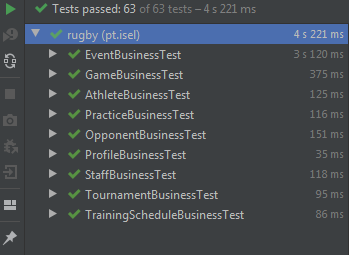
\includegraphics{./figures/tests.png}}
	\end{center}
	\caption{Demonstração de todos os testes da aplicação servidora a concluirem com sucesso.}\label{fig:gamessortednameup}
\end{figure}
\newpage
\section{Aplicação Cliente}\label{sec52}
Todos os testes feitos à aplicação cliente foram executados com ligação direta à \textit{web API} exposta pela aplicação servidora. Todos os exemplos e demonstrações apresentados ao longo do Capítulo 4 têm como base informação que provem diretamente das chamadas aos \textit{endpoints} da aplicação servidora, e toda a aplicação cliente foi testada com esses dados.

% Capitulo 6
% !TeX spellcheck = pt_PT
%
% Capítulo 6
%
\chapter{Conclusão} \label{conclusao}
Este capítulo descreve as conclusões que foram adquiridas do trabalho feito até ao momento.

\section{Recapitulação}\label{sec61}
Como referido na secção 2.1, foi possível, através de reuniões com clubes deste desporto, definir as propriedades principais e secundárias da nossa aplicação. Após estas propriedades estarem definidas e estruturadas, foi gerado o modelo de entidades onde assenta a nossa aplicação (demonstrado no Apêndice A).

Todo o trabalho feito até agora foi maioritariamente do lado da aplicação servidor. Como referido no capítulo 3, foram definidas todas as estruturas, tanto em termos de entidades e informação persistente, como em termos do formato em que a aplicação no geral irá ter acesso a esta informação. Distribuindo os focos principais nas camadas de Modelo, Repositório, Negócio e Controlador, podemos de uma forma organizada separar todo o processo que envolve o caminho desde o \emph{browser} até à base de dados. Com o auxílio das ferramentas apresentadas na secção 2.3, conseguimos organizar toda esta partição e mantê-la consistente. 

Do lado da aplicação cliente, como apresentado no capítulo 4, foram apenas geradas as classes que correspondem às classes de Entidades da aplicação servidor.

Todos os testes feitos foram ao lado da aplicação servidor. Podemos observar o comportamento dos \emph{endpoints} e a persistência dos dados na base de dados.

% Referências
%\bibliographystyle{unsrt}
%\bibliography{referencias}
%\addcontentsline{toc}{chapter}{Refer\^{e}ncias}

% Apêndices (opcional)
\appendix
% !TeX spellcheck = pt_PT
%
%
% Apêndice 1
%
\chapter{Apêndice A} \label{ap:exemplo}
O Apêndice A contem a lista de todas as entidades e as suas propriedades. 

A lista de entidades representa as propriedades que são tipos primitivos pelo seu nome(id,height,weight), as propriedades que referem associações de um para um pelo nome da entidade a que está associada(\emph{Profile}), e as propriedades que referem associações de um para muitos por uma lista de entidades a que está associada(List$<$\emph{Event}$>$).


Lista de Entidades
\begin{enumerate}
	\item \emph{Athlete}	(id,height,weight,athleteNumber,comment,\emph{Profile},List$<$\emph{Practice}$>$,List$<$\emph{TrainingSchedule}$>$,
	List$<$\emph{Game}$>$,List$<$\emph{AthleteGameStats}$>$)
	\item \emph{AthleteGameStats} (id,\emph{Athlete},\emph{Stats},\emph{Game})
	\item \emph{Event} (id,name,description,date,local,List$<$\emph{Profile}$>$)
	\item \emph{Game} (id,date,local,comment,\emph{Opponent},List$<$\emph{Athlete}$>$,List$<$\emph{AthleteGameStats}$>$)
	\item \emph{Opponent}
	(id,name,photo)
	\item \emph{Practice} (id,date,local,comment,List$<$\emph{Athlete}$>$)
	\item \emph{Profile} (id,name,birth,address,mail,phone,photo,List$<$\emph{Event}$>$)
	\item \emph{Staff} (id,staffNumber,\emph{Profile},\emph{StaffType})
	\item \emph{StaffType}(id,name)
	\item \emph{Stats} (id,errors,fouls,turnOvers,yellowCards,redCards,tries,mauls,playingTime,\emph{Tackle},\emph{Mellee},\\
	\emph{ConvertionKick},\emph{GoalKick},\emph{DropKick},\emph{OffSide},\emph{LineOut},List$<$\emph{AthleteGameStats}$>$)
	\item \emph{Tackle} (tackleHits,tackleMiss)
	\item \emph{Mellee} (melleeHits,melleeMiss)
	\item \emph{ConvertionKick} (convertionKickHits,convertionKickMiss)
	\item \emph{GoalKick} (goalkickHits,goalkickMiss)
	\item \emph{DropKick} (dropKickHits,dropkickMiss)
	\item \emph{OffSideKick} (offsideHits,offsideMiss)
	\item \emph{LineOut} (lineOutHits,lineOutMiss)
	\item \emph{Tournament} (id,classification,comment)
	\item \emph{TrainingSchedule} (id,description,link,date,List$<$\emph{Athlete}$>$)
\end{enumerate}
Todas estas entidades foram implementadas diretamente na camada do Modelo.
\newpage

\end{document} 